\documentclass[aspectratio=1610]{beamer}
\mode<presentation> {

\setbeamertemplate{navigation symbols}{}

}
\hypersetup{
        unicode=true,
        linkcolor=blue,
        anchorcolor=blue,
        citecolor=green,
        filecolor=black,
        urlcolor=blue
    }

%%%%% PACKAGES HERE
%% \usepackage{}
\usepackage{amsmath}
\usepackage{amssymb}
\usepackage{listings}
\usepackage[cache=false]{minted}
\usepackage{textcomp}
\usepackage{tikz}
\usetikzlibrary{trees}

\usepackage[style=authortitle,backend=biber]{biblatex}
\addbibresource{references.bib}

%% Start from here.
\title{How does public transportation affect household finances?}
\author{Kyra Sadovi}
\date\today

\begin{document}
%%
\begin{frame}[plain]
  \titlepage
\end{frame}

%%
\begin{frame}{Outline}
  \tableofcontents
\end{frame}
%%%%%%%%%%%%%%%%%%%%%%%%%%%%%%
\section{Proposed Research Agenda}
%%
\begin{frame}
  \tableofcontents[currentsection, subsectionstyle=show/show/hide]
\end{frame}
%%
\subsection{Research Agenda}

\begin{frame}
  \begin{center}
      \Large{How does access to public transit affect household finances?} 
  \end{center}
\end{frame}

\begin{frame}{Research Agenda}
    \begin{center}
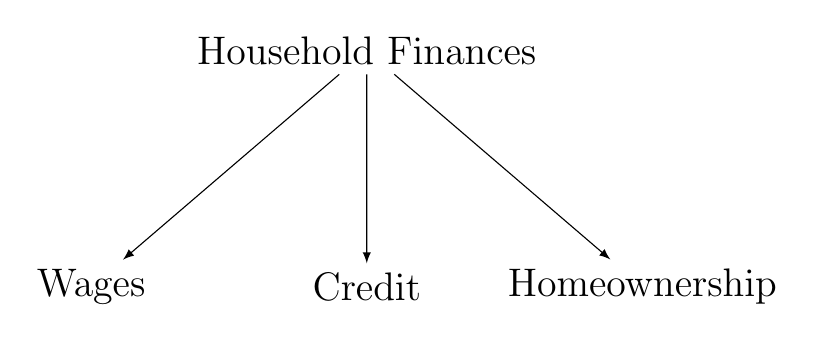
\begin{tikzpicture}
    [
    grow=south, sibling distance=35mm, level distance=30mm,
    edge from parent/.style={draw,-latex},
    every node/.style={font=\Large, align=center}
    ]
    
    \node {Household Finances}
        child { node {Wages} }
        child { node {Credit} }
        child { node {Homeownership} };
\end{tikzpicture}
\end{center}
\end{frame}

\subsection{Policy Implications}
\begin{frame}{Policy Implications}
    \begin{itemize}
        \item Gain intuition for how public transportation affects residential areas
        \begin{itemize}
            \item What is the amenity value of public transportation?  
            \item In what types of areas is public transportation most useful?
            \item What return are cities getting from investment in public transit?  
        \end{itemize}
        \item Inform public transit strategies
        \begin{itemize}
            \item Where should cities locate stations? 
            \item Where does public transit take-up have the largest effect on household welfare? 
        \end{itemize}
    \end{itemize}
\end{frame}

\subsection{Intellectual/Literature Implications}
\begin{frame}{Intellectual/Literature Contributions}
    \begin{itemize}
        \item Spatial literature 
        \begin{itemize}
            \item How do local networks improve with transit access? 
            \item Does information access (financial literacy) improve with physical mobility? 
        \end{itemize}
        \item Transportation literature
        \begin{itemize}
            \item How should we grapple with incumbency when measuring transit changes? 
            \item Individual vs. spatial unit of focus
        \end{itemize}
    \end{itemize}
\end{frame}
%%%%%%%%%%%%%%%%%%%%%%%%%%%%%%
\section{Today's Focus}
%%
\begin{frame}
  \tableofcontents[currentsection, subsectionstyle=show/show/hide]
\end{frame}
%%

\begin{frame}{}
      \begin{center}
      \Large{Does increased access to public transit affect local wages?} 
  \end{center}
\end{frame}

%%%%%%%%%%%%%%%%%%%%%%%%%%%%%%
\section{Relevant Papers}
%%
\begin{frame}
  \tableofcontents[currentsection, subsectionstyle=show/show/hide]
\end{frame}
%%

\begin{frame}{Papers}
    \begin{itemize}
        \item Households with access to cars have better employment outcomes.\footcite{RAPHAEL2002109} Implications for mobility. 
        \item Many papers on the spatial mismatch hypothesis point to public transit as a critical good for low-income and carless households.\footcite{Sanchez}
        \item Physical mobility has a large impact on referral effects in the job market.\footcite{patacchini}
        \item There are already some papers studying this, but are limited in scope\footcite{TYNDALL2021103350}
    \end{itemize}
\end{frame}

%%%%%%%%%%%%%%%%%%%%%%%%%%%%%%
\section{Econometric Approach}
%%
\begin{frame}
  \tableofcontents[currentsection, subsectionstyle=show/show/show]
\end{frame}
%%
\subsection{Econometric Challenges}
\begin{frame}{Econometric Challenges}
    \begin{block}{Anticipation Effects}
        Neighborhoods start to change well before a station opens\footcite{mcmillen2004reaction}. How do we isolate the effect of the \textbf{physical presence} of a working station? 
    \end{block}
    \begin{block}{Composition Effects}
        A neighborhood before the announcement of a station might not be the same one that exists after it opens\footcite{Pedeiro}. How can we measure the effect of this change on \textbf{incumbent residents}?
    \end{block}
\end{frame}

\subsection{Identification approach}
%%

\subsubsection{Anticipation Effects}
%%
\begin{frame}
  \tableofcontents[currentsubsection, subsectionstyle=show/show/show]
\end{frame}
%%
\begin{frame}{Anticipation Effects}
    \begin{block}{NEPA Process}
        \begin{itemize}
            \item Any transit project that receives federal funds must comply with the National Environmental Policy Act (\textbf{NEPA}) evaluation process
            \item Environmental impact statements (EIS) introduce delays
            \item The EPA's EIS database: all EIS submissions since 1987. Each reports an anticipated opening date. 
        \end{itemize}
    \end{block}
\end{frame}

\begin{frame}{Anticipation Effects}
    \begin{block}{NEPA Process}
        \begin{itemize}
            \item Any transit project that receives federal funds must comply with the National Environmental Policy Act (\textbf{NEPA}) evaluation process
            \item Environmental impact statements (EIS) introduce delays
            \item The EPA's EIS database: all EIS submissions since 1987. Each reports an anticipated opening date. 
        \end{itemize}
    \end{block}
    \begin{block}{Other Exogenous Delays}
        \begin{itemize}
            \item Acts of god (hurricanes, weather) 
            \item Political intervention (not always exogenous)
        \end{itemize}
    \end{block}
\end{frame}

\begin{frame}{Constructing a Time Index $j$}
    
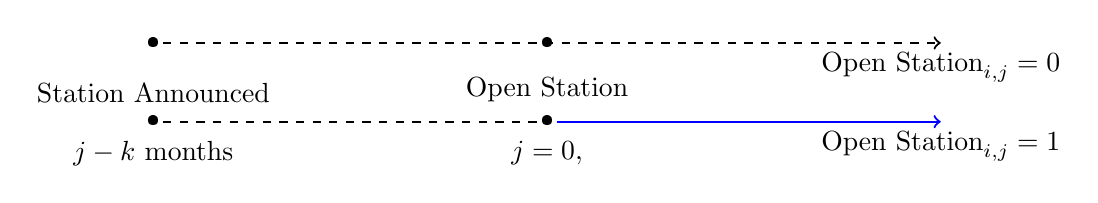
\begin{tikzpicture}

% Top arrow - Dashed
\node (A) at (0,1) {};
\draw[dashed, ->, thick] (A) -- (10,1);
\node at (0,1) {\textbullet};
\node at (5,1) {\textbullet};

% Bottom arrow - Dashed up to middle node, then solid
\node (B1) at (0,0) {};
\node (B2) at (5,0) {};
\draw[dashed, thick] (B1) -- (B2);  % Dashed part
\draw[->, thick, blue] (B2) -- (10,0);     % Solid part
\node at (0,0) {\textbullet};  % Left node bullet point
\node at (5,0) {\textbullet};  % Middle node vertical line

% Labels for the bottom arrow nodes
\node[above] at (B1.north) {Station Announced};
\node[above] at (B2.north) {Open Station};
\node[below] at (B1.south) {$j-k$ months};
\node[below] at (B2.south) {$j=0,$};
\node[below] at (10,0) {$\text{Open Station}_{i,j}=1$};
\node[below] at (10,1) {$\text{Open Station}_{i,j}=0$};

\end{tikzpicture}
\end{frame}

\subsubsection{Composition Effects}
%%
\begin{frame}
  \tableofcontents[currentsubsection, subsectionstyle=show/show/show]
\end{frame}
%%
\begin{frame}{Composition Effects}
    \begin{block}{Individuals as a unit of measure}
        \begin{itemize}
            \item Many obstacles faced in other papers are related to limitations of this type
            \item Most other papers use neighborhoods as their unit of measure, making this a problem 
            \item Focusing on the individual allows us to identify incumbents and measure their welfare after such infrastructure improvements 
            \item LEHD: track residential location and labor market outcomes over time
        \end{itemize}
    \end{block}
    \begin{block}{Potential problems}
    \begin{itemize}
        \item Renters are frequently mobile, and tenure in a neighborhood matters for measuring impact. Need to figure out a way to identify long-term neighborhood residents (or do I)? 
        \item Homeowners are much more ``locked-in'' than their renting counterparts. My incumbents may be biased toward homeownership if I require long tenure in a neighborhood. 
    \end{itemize}
    \end{block}
\end{frame}

\subsection{Model}
%%
\begin{frame}
  \tableofcontents[currentsection, subsectionstyle=show/show/hide]
\end{frame}
%%
\begin{frame}{Model}
    $$Wages_{i,j}=\beta_k\text{Open Station}_{i,j}+\theta_k+\gamma_j+X_i+\varepsilon_{i,j}$$
    \begin{columns}[c] % The "c" option specifies centered vertical alignment while the "t" option is used for top vertical alignment

        \column{0.4\textwidth}
        Subscripts
            \begin{itemize}
                \item $i$: Individual
                \item $j$: Time period 
                \item $k$: Neighborhood type 
            \end{itemize}

        \column{0.5\textwidth}
        Regressors
            \begin{itemize}
                \item $\text{Open Station}_{i,j}$: Dummy for person $i$ in period $j$
                \item $\theta_k$: Neighborhood fixed effects 
                \item $\gamma_j$: Period fixed effects
                \item $X_{i,j}$: Worker-level controls
            \end{itemize}
    \end{columns}
\end{frame}

%%%%%%%%%%%%%%%%%%%%%%%%%%%%%%
\begin{frame}[noframenumbering,plain,allowframebreaks]{References}
    \printbibliography[heading=none]
\end{frame}

\end{document}